\chapter{Discussion}
Please tell more about conclusion and how to the next work of this study.

\section{Imron Sumadireja / 1164076}
\subsection{Teori}
\begin{enumerate}

\item Jelaskan kenapa file suara harus di lakukan MFCC. Dilengkapi dengan ilustrasi atau gambar. \par
MFCC merupakan koefisien yang merepresentasikan audio. Ekstraksi ciri dalam proses ini ditandai dengan pengubahan data suara menjadi citra berupa spektrum gelombang. File audio dilakukan MFCC itu agar objek suara dapat diubah menjadi bentuk matrix. Suara tersebut akan menjadi vektor yang nantinya akan diolah sebagai keluaran. Untuk ilustrasi sederhananya bisa dilihat pada gambar \ref{cc1}. Gambar tersebut menjelaskan tahapan-tahapan kenapa file suara harus dilakukan MFCC. Selain itu untuk memberikan kemudahan kepada mesin dalam mempelajari suara tersebut karena mesin tidak dapat membaca teks maka dari itu diperlukan MFCC untuk merubah suara tersebut menjadi vektor.
		\begin{figure}[!htbp]
		\centerline{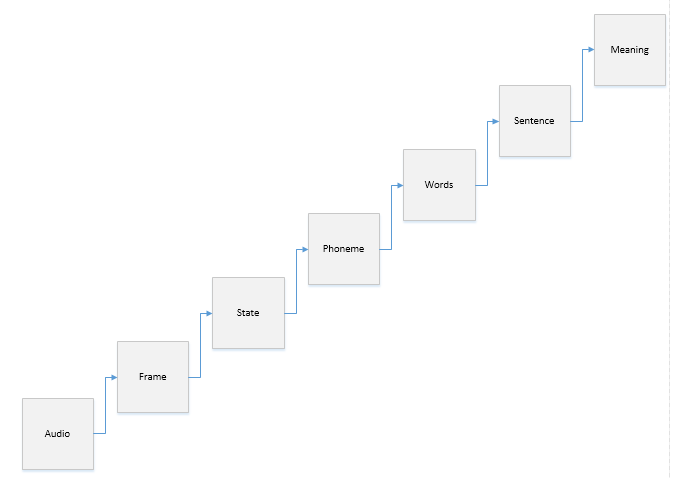
\includegraphics[width=0.5\textwidth]{figures/im/cc1.png}}
		\caption{MFCC.}
		\label{cc1}
		\end{figure}

\item Jelaskan konsep dasar neural network. Dilengkapi dengan ilustrasi atau gambar. \par
Konsep sederhana dari neural network hampir mirip dengan proses belajar pada anak-anak yakni dengan memetakan pola baru yang didapatkan dari inputan untuk membuat pola baru pada keluaran. Contoh sederhana tersebut menganalogikan kinerja otak manusia. Neural network itu sendiri terdiri dari sebuah unit pemroses yang disebut neuron yang berisi adder dan fungsi aktivasi. Fungsi aktivasi itu sendiri untuk mengatur keluaran yang diberikan oleh neuron. Neural network ini mengadopsi mekanisme berpikir sebuah sistem atau aplikasi yang menyerupai otak manusia, baik untuk pemrosesan berbagai sinyal elemen yang diterima, toleransi terhadap kesalahan/error, dan juga prallel processing. Karakteristik dari neural network dilihat dari pola hubungan antar neuron, metode penentuan bobot dari tiap koneksi, dan fungsi aktivasinya. Untuk ilustrasinya bisa dilihat pada gambar \ref{cc2}
		\begin{figure}[!htbp]
		\centerline{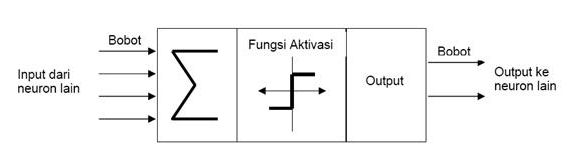
\includegraphics[width=0.5\textwidth]{figures/im/cc2.png}}
		\caption{Konsep Dasar Neural Network.}
		\label{cc2}
		\end{figure}

\item Jelaskan konsep pembobotan dalam neural network. Dilengkapi dengan ilustrasi atau gambar. \par
Pembobotan ini akan menentukan serta penanda dari sebuah konektivitas. Pada proses neural network dimulai dari input yang diterima oleh neuron beserta dengan nilai bobot dari tiap-tiap input yang ada. Setelah masuk ke dalam neuron, nilai input yang ada akan dijumlahkan oleh suatu fungsi penambahan. Hasil penjumlahan tersebut akan diproses oleh fungsi aktivasi oleh setiap neuron, hasil penjumlahan tersebut akan dibandingkan dengan nilai ambang tertentu. Jika nilai dari hasil penjumlahan tersebut melebihi nilai ambang maka aktivasi neuron akan dibatalkan, namun sebaliknya jika hasil penjumlahan dibawah nilai ambang maka neuron akan diaktifkan. Setelah neuron aktif selanjutnya akan mengirimkan nilai output melalui bobot-bobot keluarannya ke semua neuroon yang berhubungan. Ilustrasinya bisa dilihat pada gambar \ref{cc3}
		\begin{figure}[!htbp]
		\centerline{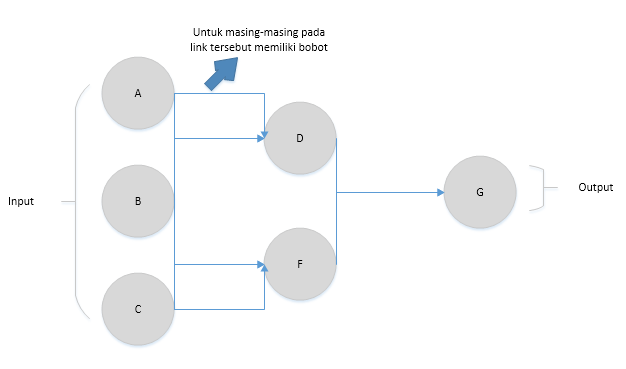
\includegraphics[width=0.5\textwidth]{figures/im/cc3.png}}
		\caption{Konsep Pembobotan Neural Network.}
		\label{cc3}
		\end{figure}

\item Jelaskan konsep fungsi aktifasi dalam neural network. Dilengkapi dengan ilustrasi atau gambar. \par
Fungsi aktivasi ini merupakan operasi matematik yang dikenakan pada sinyal output. Fungsi ini digunakan untuk mengaktifkan atau menonaktifkan neuron. Fungsi aktivasi ini terbagi setidaknya menjadi 6, dianranya sebagai berikut:
\begin{itemize}
\item a. Fungsi Undak Biner Hard Limit, fungsi ini biasanya digunakan oleh jaringan lapiran tunggal untuk mengkonversi nilai input dari suatu variabel yang bernilai kontinu ke suatu nilai output biner 0 atau 1.
\item b. Fungsi Undak Biner Threshold, fungsi ini menggunakan nilai ambang sebagai batasnya.
\item c. Fungsi Bipolar Symetric Hard Limit, fungsi ini memiliki output bernilai 1, 0 atau -1.
\item d. Fungsi Bipolar dengan Threshold, fungsi ini mempunyai output yang bernilai 1, 0 atau -1 untuk batas nilai ambang tertentu.
\item e. Fungsi Linear atau Identitas.
\end{itemize}
Untuk ilustrasi sederhananya bisa dilihat pada gambar \ref{cc4}. Gambar tersebut merupakan salah satu contoh dari fungsi aktivasi bipolar.
		\begin{figure}[!htbp]
		\centerline{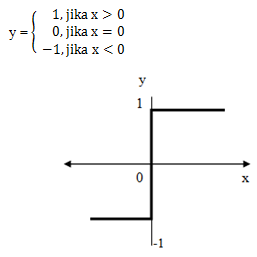
\includegraphics[width=0.5\textwidth]{figures/im/cc4.png}}
		\caption{Konsep Fungsi Aktivasi Neural Network.}
		\label{cc4}
		\end{figure}

\item Jelaskan cara membaca hasil plot dari MFCC. Dilengkapi dengan ilustrasi atau gambar. \par
Membaca plot MFCC ini bisa kita lihat pada gambar \ref{cc5}. Gambar tersebut menjelaskan bahwa pada waktu ke 5 daya atau desible yang dikelurakan pada nada tersebut paling keras pada 20 Hz, selain itu pada 40 -120 Hz itu daya atau desible yang dikeluarkan pada musik yang telah di plotting. Begitupun seterusnya bahwa warna yang paling gelap itu merupakan daya atau desible yang paling tinggi dibandingkan dengan warna yang cerah. Untuk yang berwarna merah itu suara dibawah pendengaran frekuensi manusia, jadi tidak dapat terdengar secara langsung. 
		\begin{figure}[!htbp]
		\centerline{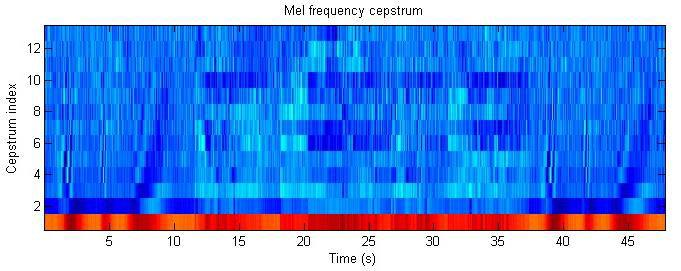
\includegraphics[width=0.5\textwidth]{figures/im/cc5.png}}
		\caption{Membaca Plot MFCC.}
		\label{cc5}
		\end{figure}

\item Jelaskan apa itu one-hot encoding. Dilengkapi dengan ilustrasi kode dan atau gambar. \par
Sederhananya one-hot encoding ini untuk merubah hasil data vektorisasi menjadi bilangan biner 0 dan 1 serta membuat keterangan pada atribut tersebut menjadi label. Unutuk ilustrasi sederhananya bisa dilihat pada gambar \ref{cc6}
		\begin{figure}[!htbp]
		\centerline{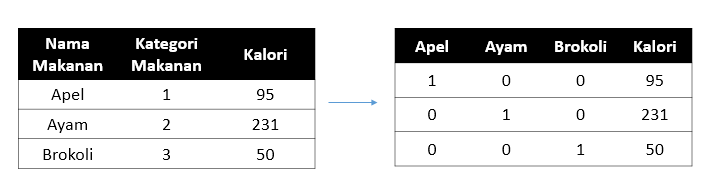
\includegraphics[width=0.5\textwidth]{figures/im/cc6.png}}
		\caption{One-Hot Encoding.}
		\label{cc6}
		\end{figure}

\item Jelaskan apa fungsi dari np.unique dan to categorical dalam kode program. Dilengkapi dengan ilustrasi atau gambar. \par
Fungsi dari np.unique adalah untuk menemukan elemen yang berbeda atau unik array, dan dapat mengembalikan elemen unik array tersebut yang diurutkan. Untuk ilustrasi sederhananya bisa dilihat pada gambar \ref{cc7}. Gambar tersebut menjelaskan bahwa unique itu sendiri akan mengambil data yang berbeda dari variabel a yang berada dalam fungsi array dan hasilnya seperti gambar tersebut.
		\begin{figure}[!htbp]
		\centerline{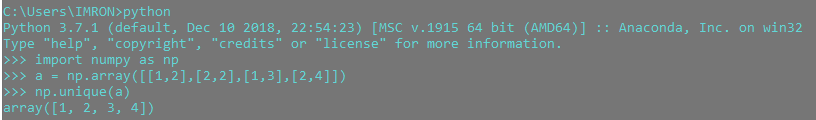
\includegraphics[width=0.5\textwidth]{figures/im/cc7.png}}
		\caption{np.unique.}
		\label{cc7}
		\end{figure}

Fungsi dari to\_categorical untuk mengubah vektor yang berupa integer menjadi matrix dengan kelas biner. Untuk ilustrasinya bisa dilihat pada gambar \ref{cc71}
		\begin{figure}[!htbp]
		\centerline{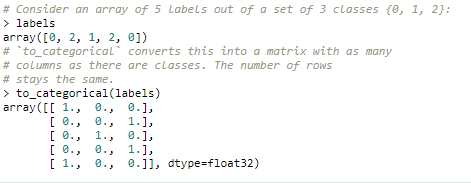
\includegraphics[width=0.5\textwidth]{figures/im/cc71.png}}
		\caption{to\_categorical.}
		\label{cc71}
		\end{figure}

\item Jelaskan apa fungsi dari Sequential dalam kode program. Dilengkapi dengan ilustrasi atau gambar.\par
Salah satu jenis model yang digunakan dalam perhitungan. Sequential ini membangun tumpukan linear yang berurutan. Contoh sederhananya sebagai berikut \ref{cc8}
		\begin{figure}[!htbp]
		\centerline{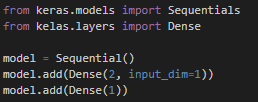
\includegraphics[width=0.5\textwidth]{figures/im/cc8.png}}
		\caption{Sequential.}
		\label{cc8}
		\end{figure}

\end{enumerate}